
\begin{section}{Project Description}
This project compares the performance, area and energy of different memory hierarchy configurations by building a flexible cache and memory simulator. A subset of the SPEC-2000 benchmark suite is used for the comparison.
\end{section}


\begin{section}{Results}

    \begin{subsection}{Effect of Size and Associativity on Miss Rate without L2 Cache}
    Intuitively, increasing cache size is expected to decrease the miss rate as there would be fewer conflict misses. A more associative cache is also expected to decrease the miss rate because it offers more flexibility, as an incoming block can be placed in more number of locations in the cache.

    \begin{figure}[h!]
        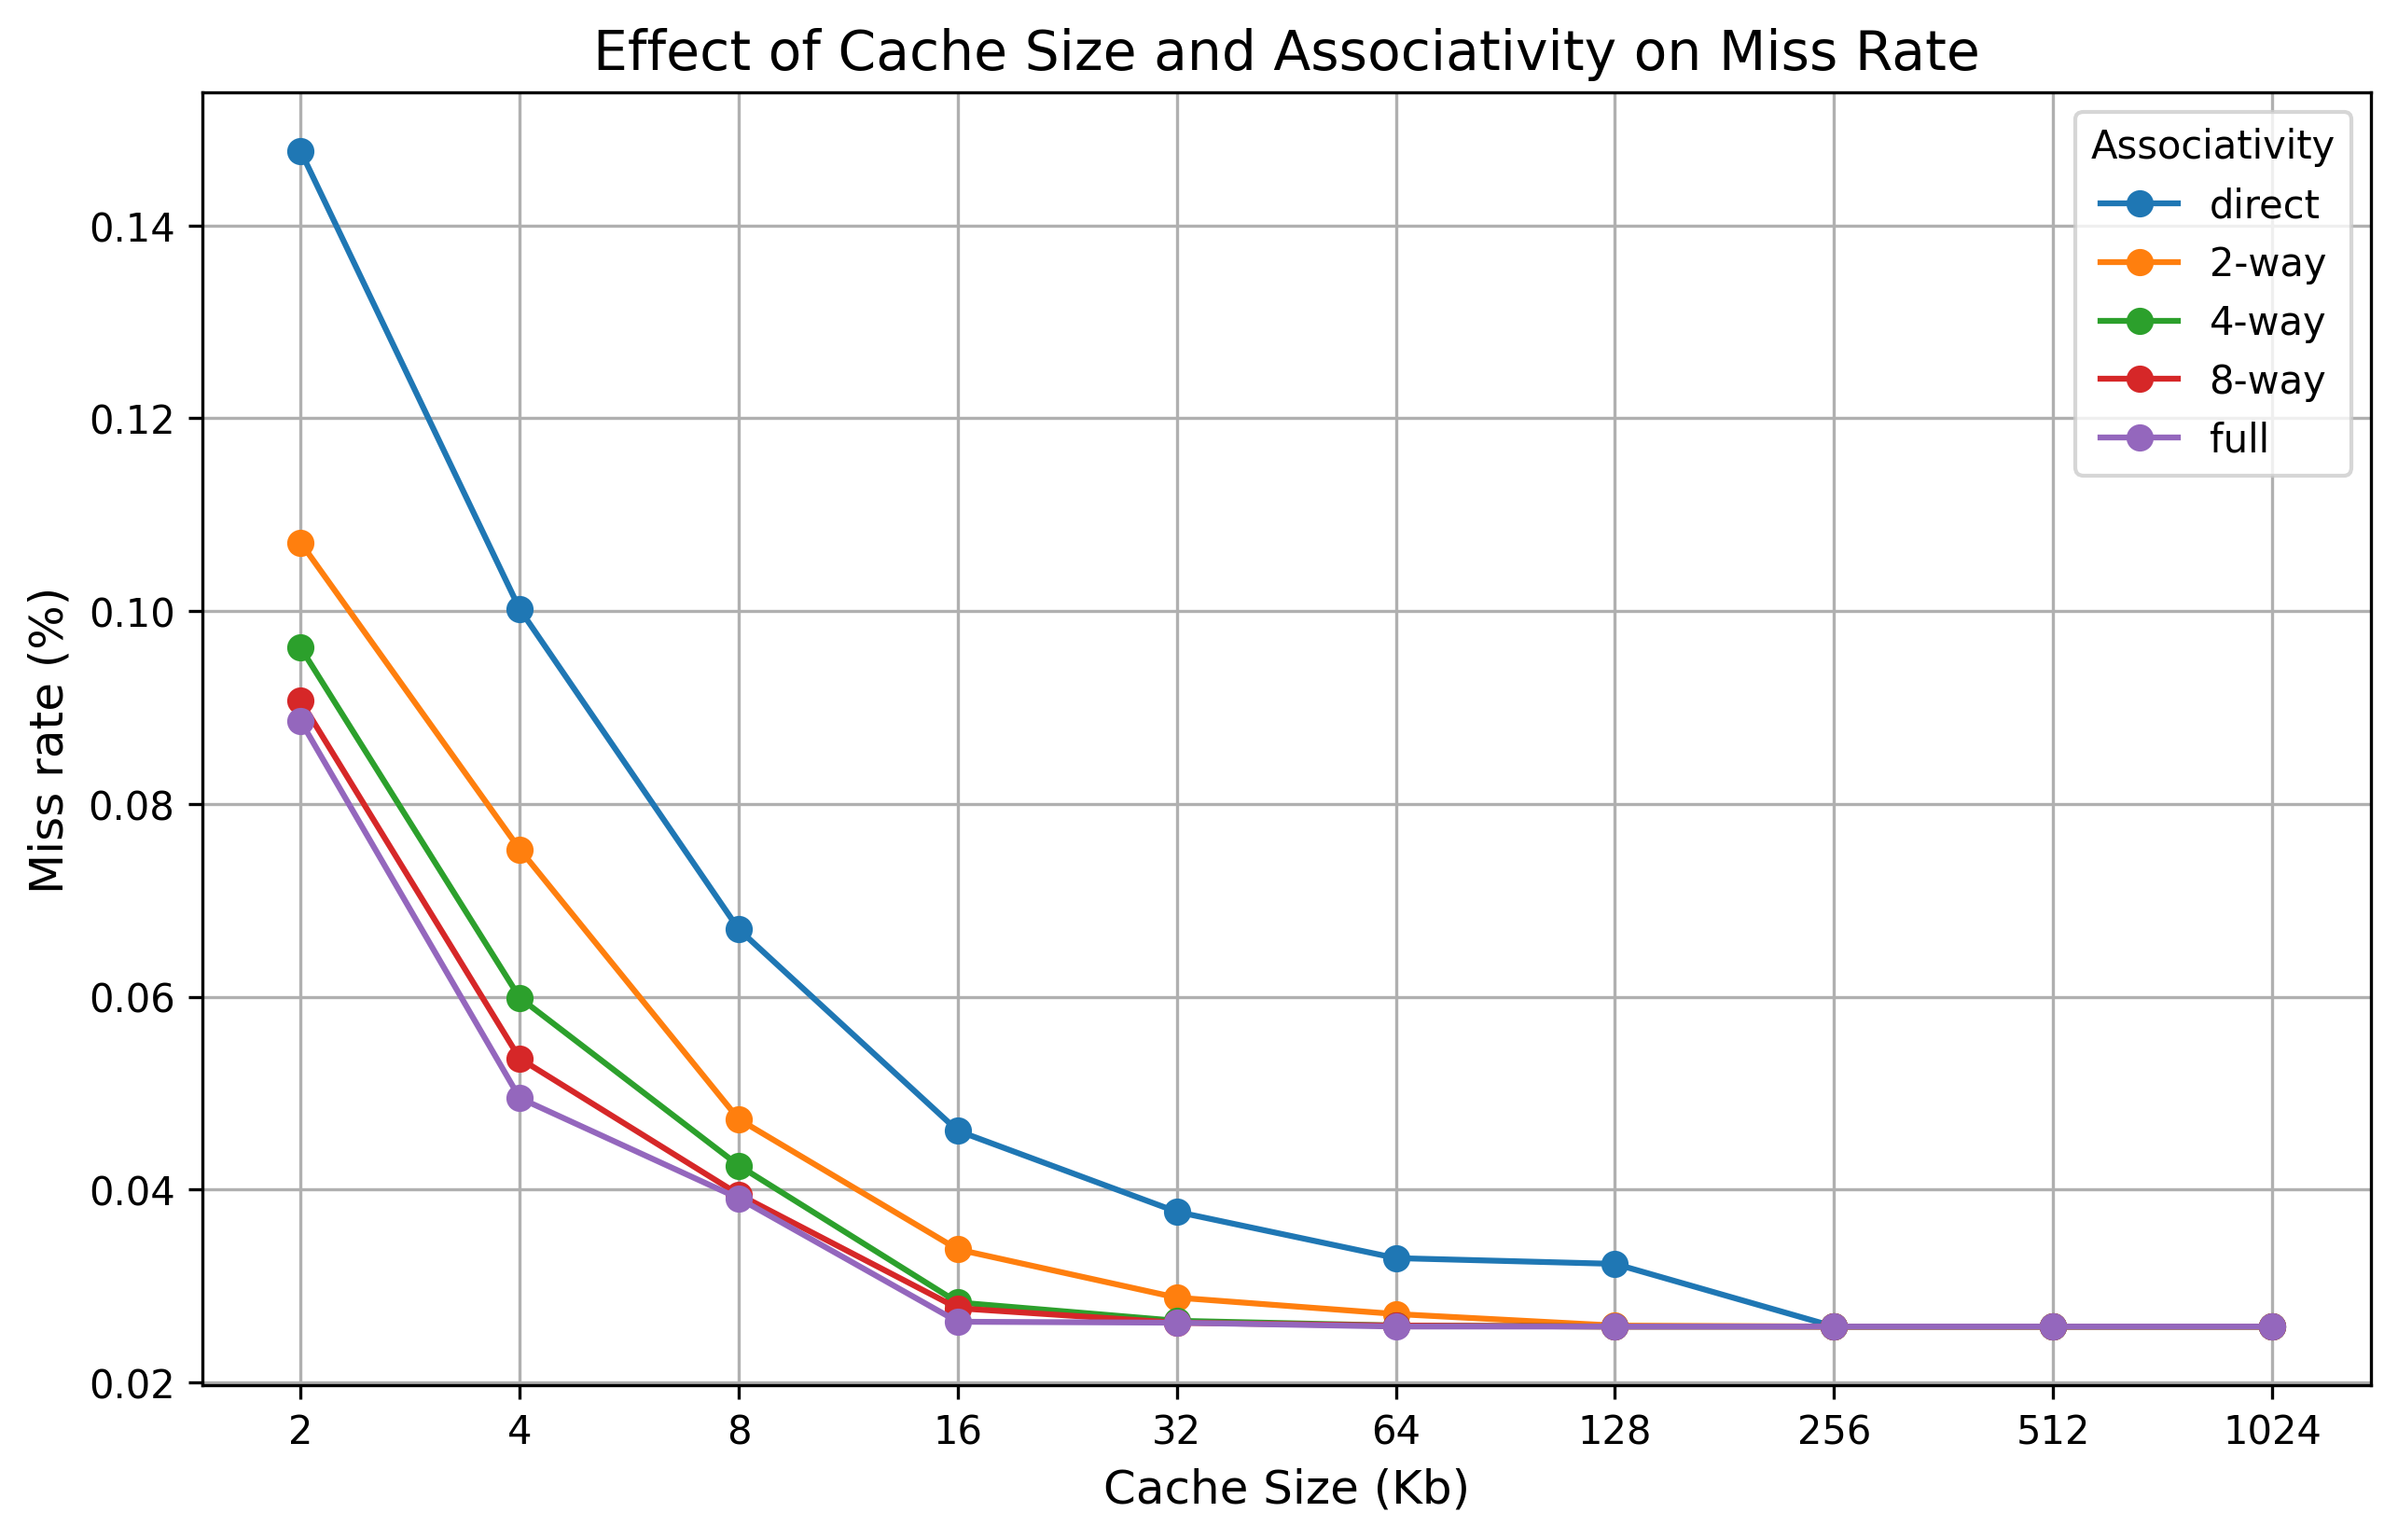
\includegraphics[width=0.9\textwidth]{figures/fig1/fig1.png}
        \centering
        \label{fig:fig1}
    \end{figure}

    \begin{subsubsection}{Trends in the graph}
    As depicted in \ref{fig:fig1}, increasing the cache size always decrease the miss rate irrespective of the associativity. Further increasing the  associativity of a fixed sized cache decreases the miss rate. However, diminishing returns were observed on increasing the associativity. For all cache sizes greater than 4 KB, a 4-way set-associative cache performed nearly as well as a fully associative cache. Another observation here is that the benefits of increasing associativity are more prominent in a smaller cache. For example, a 2-way set associative cache decreased the miss rate by nearly 30\% for a 2KB cache, but decreased it only by 20\% for a 128KB cache.
    \end{subsubsection}

    \begin{subsubsection}{Estimating Compulsory Miss rate}
    For larger fully associative caches, the miss rate converges to \textbf{0.258}, as can be seen from figure \ref{fig1}. This reflects the compulsory miss rate  of the benchmarks, because the for larger caches, capacity and conflict misses can be safely ignored. This is because, for a large fully associative cache (say 1Mb), there would always be stale blocks (which will not be accessed in the future) waiting to be removed. 
    \end{subsubsection}

    \begin{subsubsection}{Estimating the Conflict Miss rates}
    We know that all cache misses comprise of compulsory, conflict and capacity misses. However, we already know that a fully associative cache has no conflict misses. This means that we can approximate the conflict misses for a given associativity by subtracting the miss rate of a fully associative cache of the same size from the total miss rate of the cache of the same associativity and size. 
    \end{subsubsection}

    \begin{table}[h!]
        \centering
        \begin{tabular}{lcccc}
            \toprule
            \textbf{Cache Size} & \textbf{2KB} & \textbf{8KB} & \textbf{32KB} & \textbf{256KB} \\
            \midrule
            Direct-Mapped  & 5.91\% & 5.07\% & 1.15\% & 0\%\\
            2-way  & 1.85\%  & 0.82\% & 0.26\% & 0\%\\
            4-way  & 0.76\%  & 0.34\% & 0.02\% & 0\%\\
            8-way  & 0.19\% & 0.04\%  & 0\% & 0\%\\
            Fully-Associative & 0\%  & 0\% & 0\% & 0\%\\
            \bottomrule
        \end{tabular}
        \caption{Conflict miss rates for different configurations}
        \label{tab:miss_rates}
    \end{table}

    \end{subsection}

   

    \begin{subsection}{Effect of Cache Size and Associativity on Average Access Time (AAT) without L2 cache }
        There are two opposing factors that determine the effect of Cache Size and Associativity on the Average Access Time. Firstly, a larger or more associative cache requires more logic gates and has a longer critical path. This causes an increase in the hit time of the cache. However, from section 2.1, we observed that the miss rate decreases for a larger or more associative cache. This decreases the number of times the cache has to wait for the next level of memory hierarchy, which is usually much slower.

        \begin{figure}[h!]
            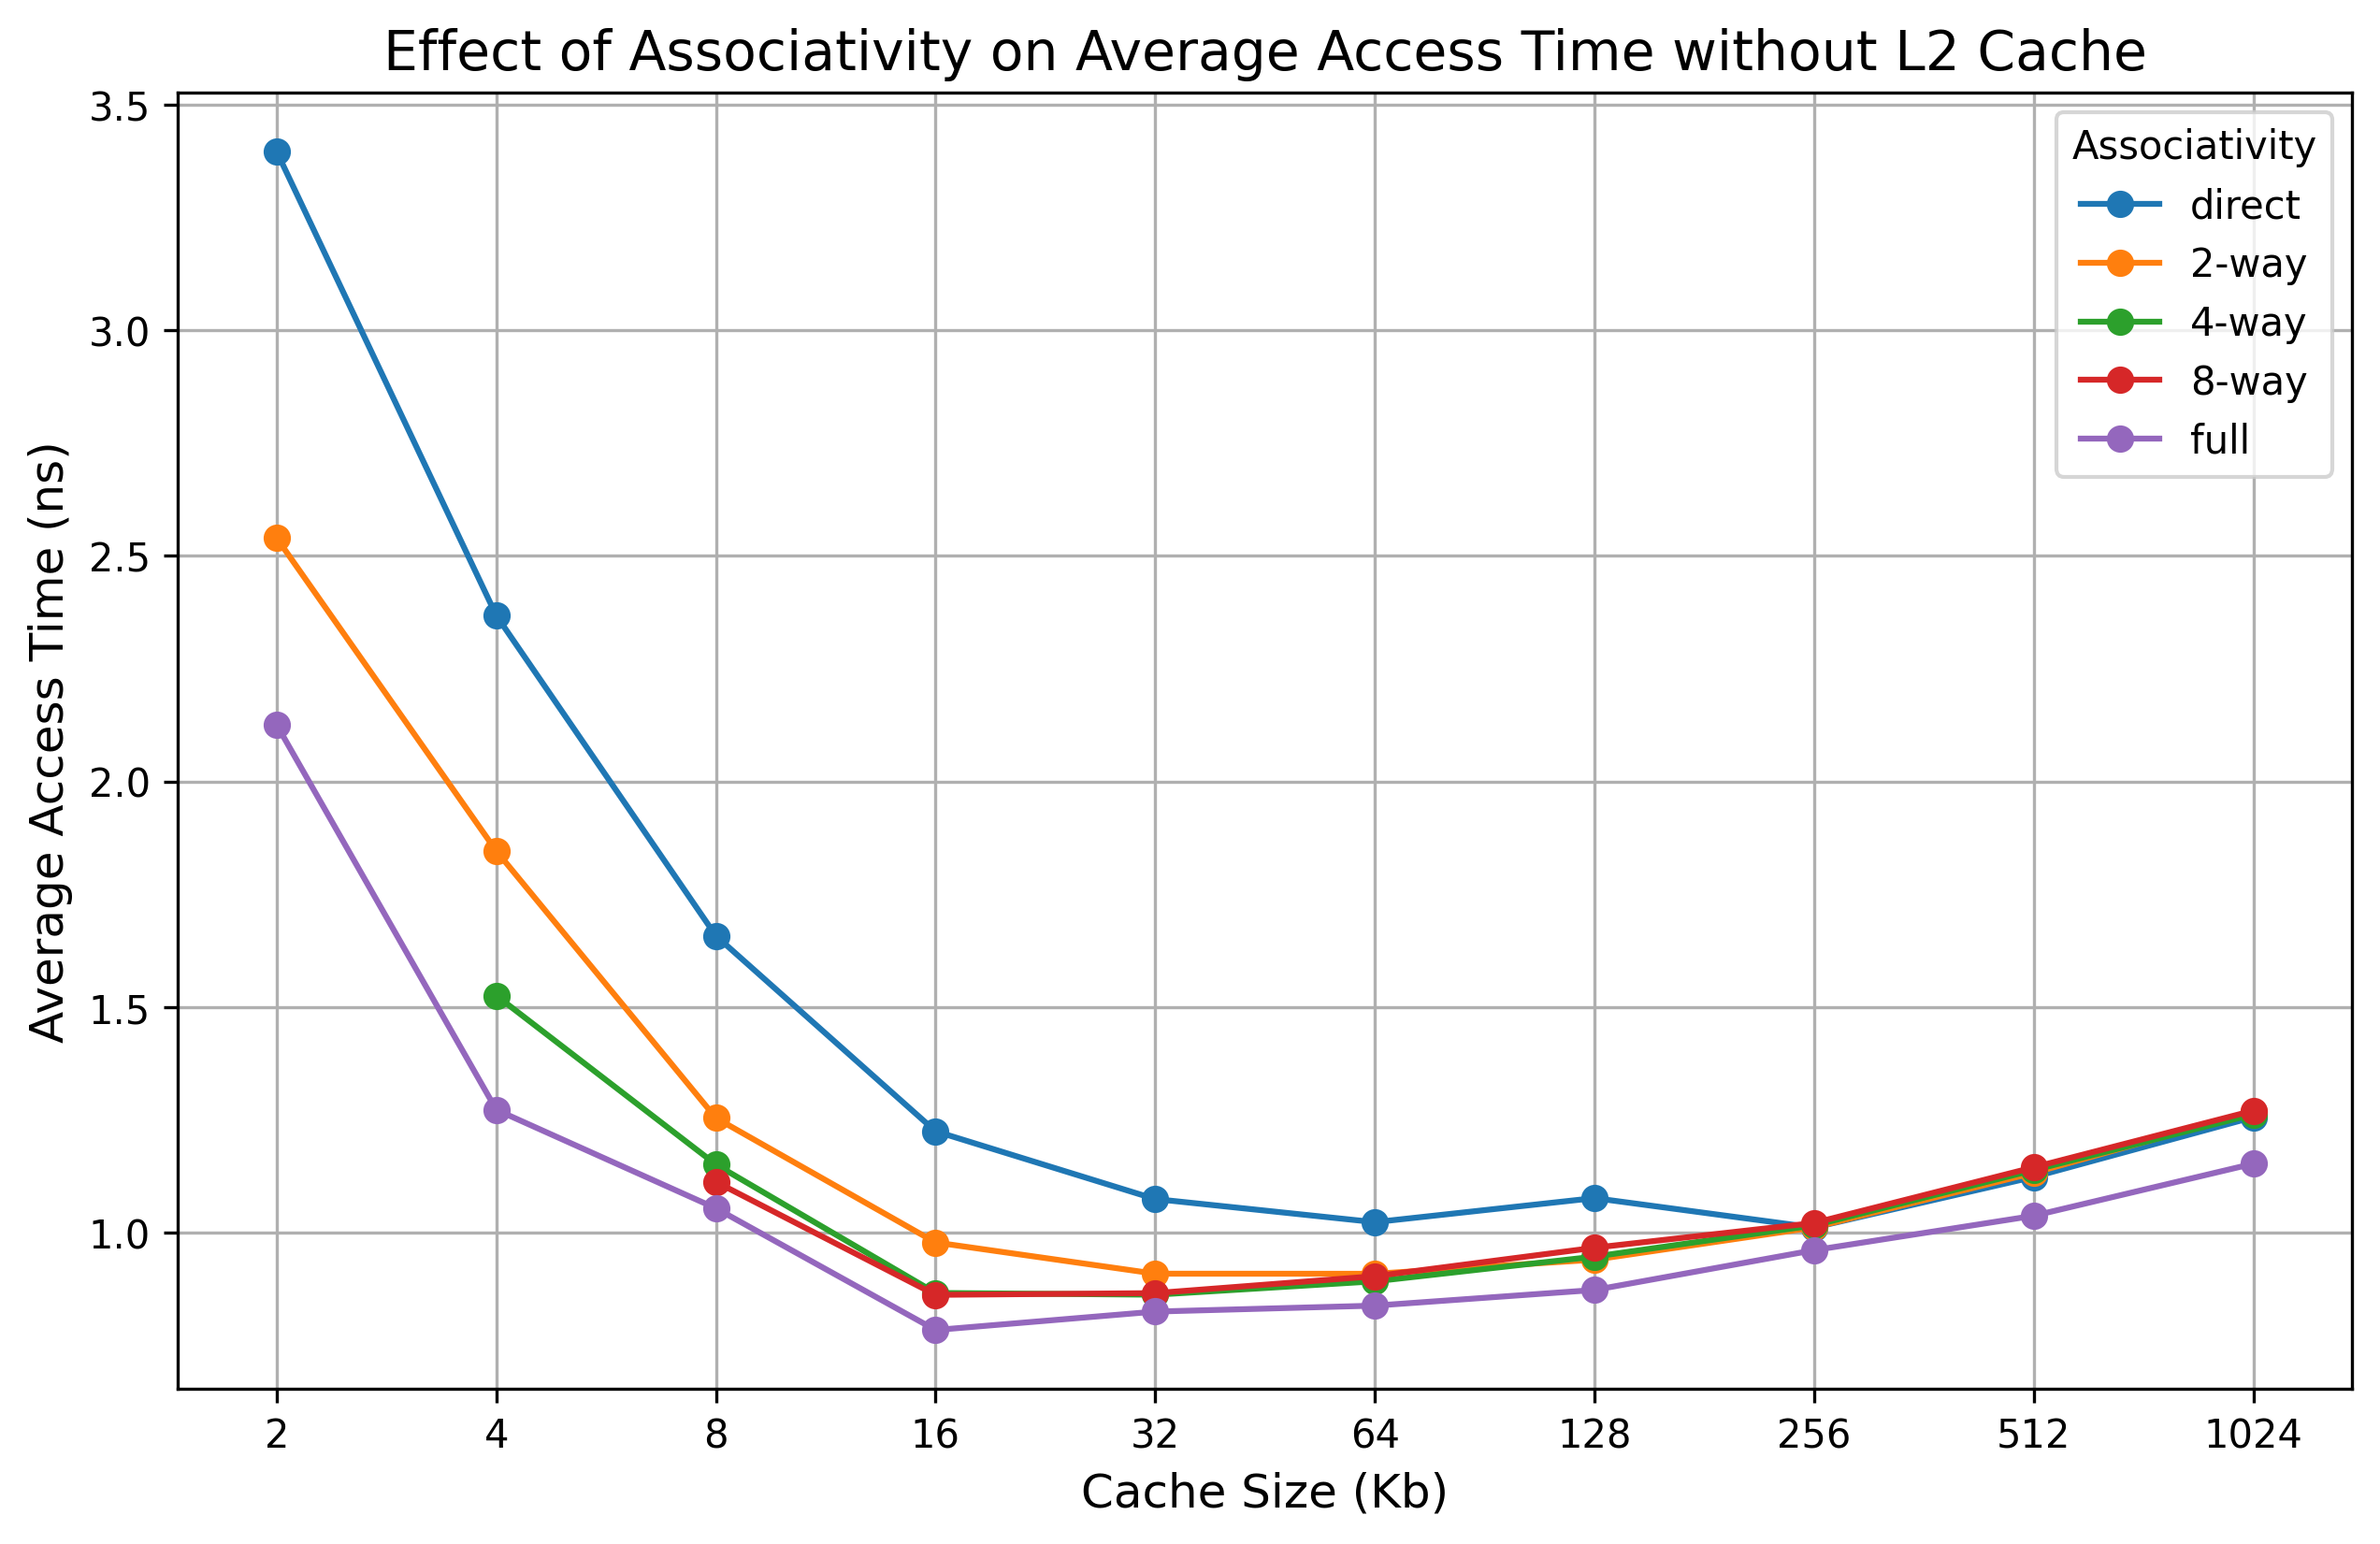
\includegraphics[width=0.9\textwidth]{figures/fig2/fig2.png}
            \centering
            \label{fig:fig2}
        \end{figure}

        From the diagram shown, \textbf{a fully associative 16KB cache} has the lowest AAT of \textbf{0.7842 ns}.
    \end{subsection}

    \begin{subsection}{Effect of Cache Size and Associativity on Average Access Time (AAT) with L2 cache}
    
        With L2 cache the second effect, as discussed above, of reducing the miss rate has lesser impact on decreasing the average access time, because a faster lower level of memory in the hierarchy has reduced miss penalty.
        
        \begin{figure}[h!]
            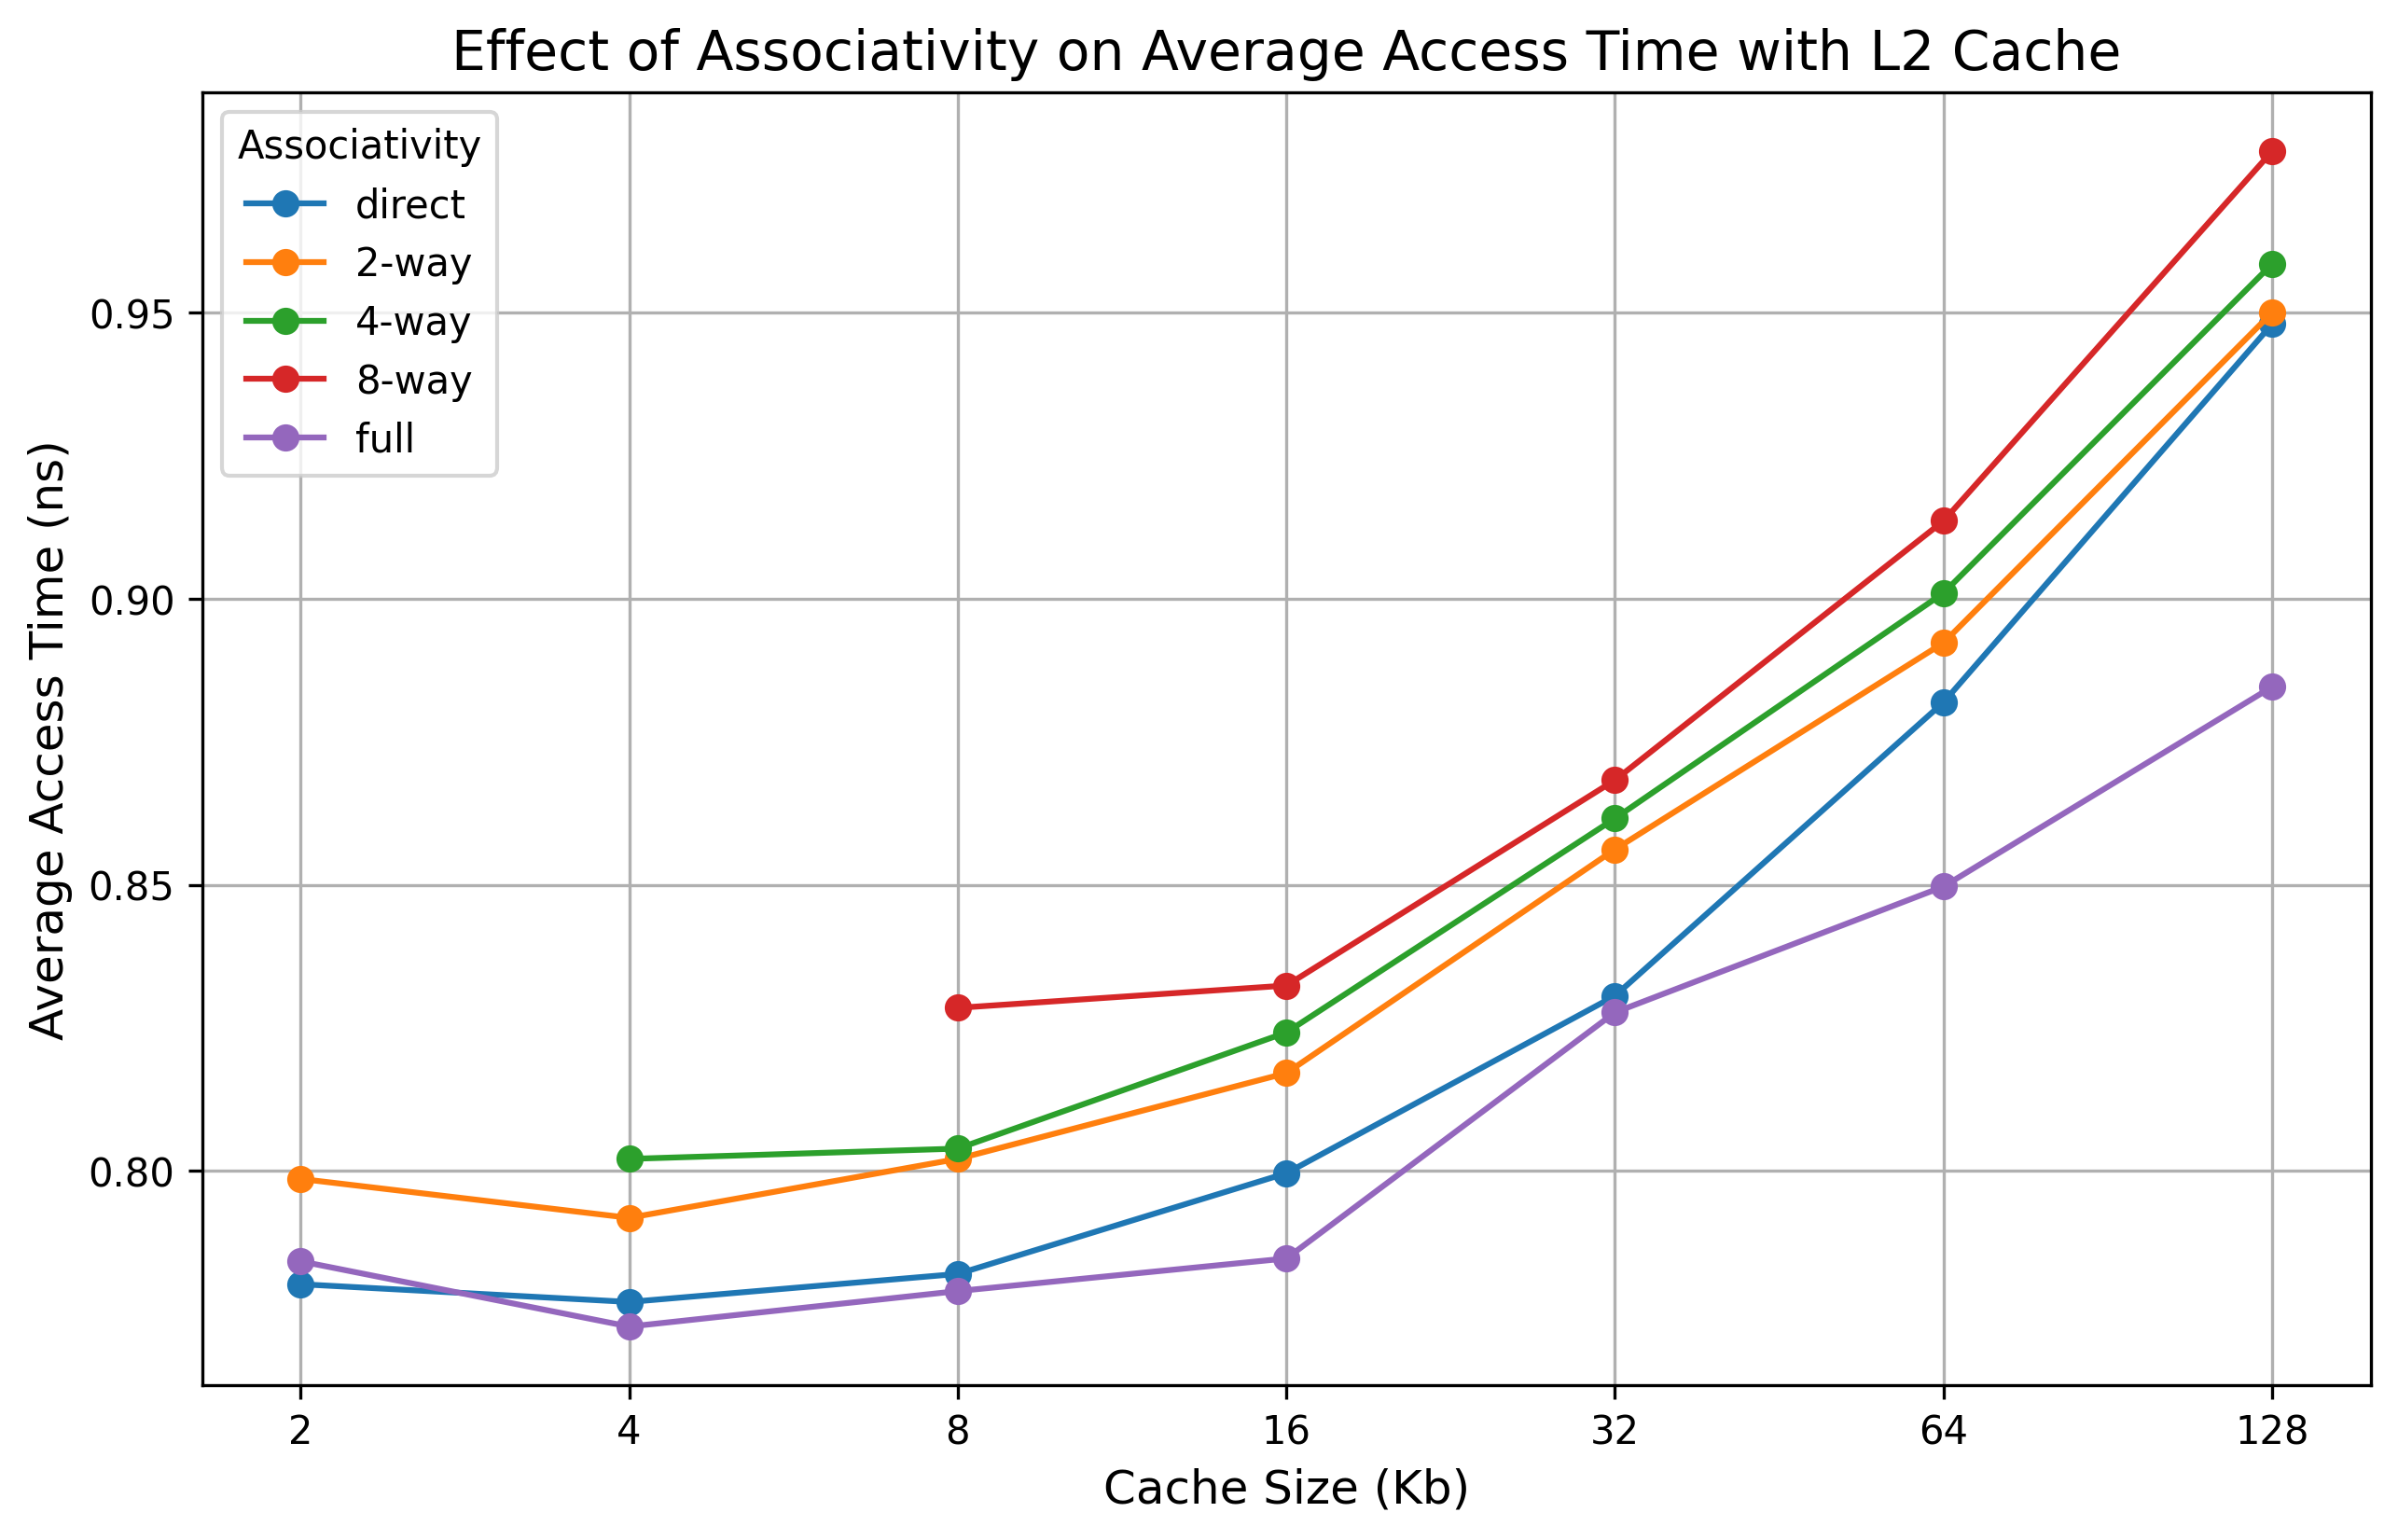
\includegraphics[width=0.9\textwidth]{figures/fig3/fig3.png}
            \centering
            \label{fig:fig3}
        \end{figure}

        With a 8-way set associative 256KB L2 cache, the lowest average acess time was observed with a \textbf{fully associative 4KB L1 cache}. This configuration had a L1 miss rate of 0.7728 ns compared to 0.7842 ns of the best configuration without a L2 cache, which is \textbf{approximately a 1.5\% reduction} in the average access time. Further this configuration has a total area of $1.1784 \text{mm}^2$ and Energy-Delay Product (EDP) of 147.82 pico J$\cdot$s compared to an total area of $0.0634 \text{mm}^2$ and EDP $460.72$ pico J$\cdot$s of the best configuration without a L2 cache. Clearly, adding a L2 cache increases the area requirement by approximately 20 fold.
        
    
    \end{subsection}

   
    \begin{subsection}{Effect of Block and Cache Sizes on Miss Rate}

    The figure below shows the miss rate of a 4-way associative L1 cache for various block and cache sizes.

    \begin{figure}[h!]
        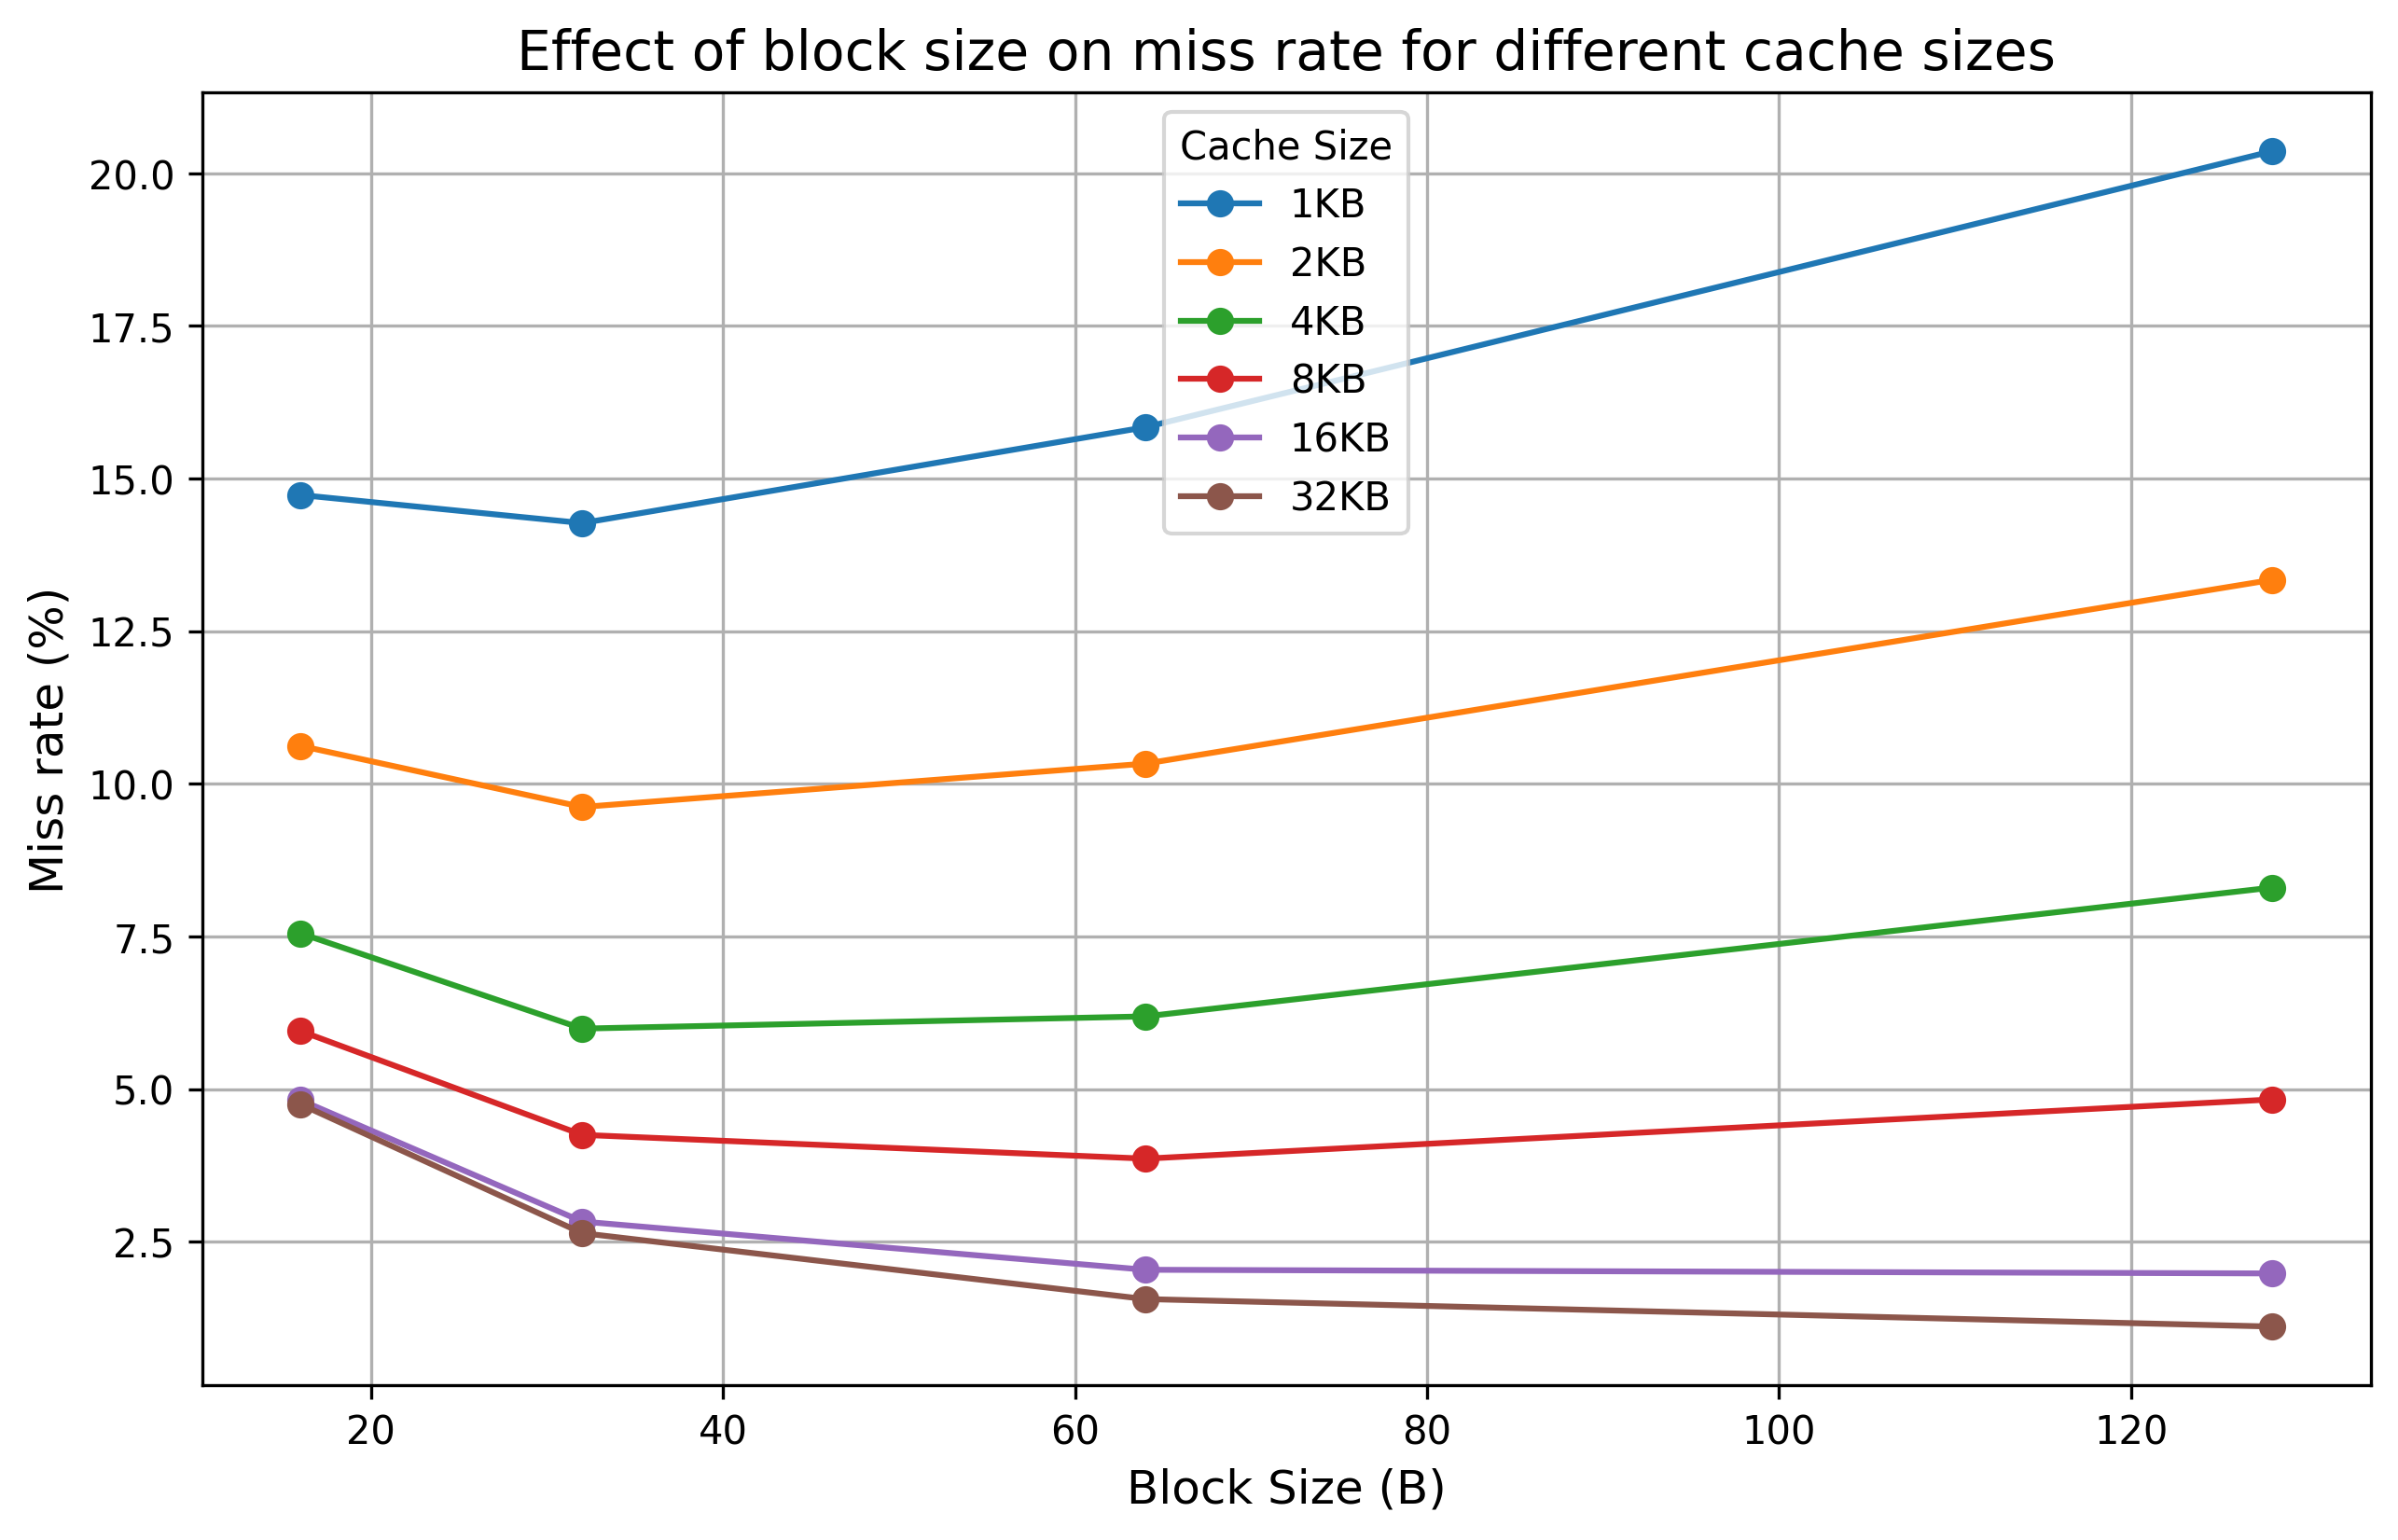
\includegraphics[width=0.9\textwidth]{figures/fig4/fig4.png}
        \centering
        \label{fig:fig4}
    \end{figure}

    There are two opposing factors that influence the effect of blocksize on the miss rate of the cache. Firstly with a bigger blocksize, more bytes are brought from the next level of memory hierarchy leading to lesser misses subsequently. This effect is stronger for programs with considerable spatial locality. On the other hand, when a bigger block is brought from memory but its bytes/words are not accessed, cache space is utilized to store unnecessary blocks, leading to cache pollution and higher miss rates. Thus the competing effects of spatial locality and cache pollution determines the overall miss rate.\\
    This effect can be observed in figure \ref{fig4}, where for a 2KB cache, a 32B blocksize performs better than 16B blocksize due to spatial locality, but a 128B blocksize performs much worse because of the overpowering cache pollution.\\
    Further, this \textbf{tradeoff between spatial locality and cache pollution is affected by cache size} as well. As the cache size increases the effects of cache pollution due to larger block size also reduces considerably, and increasing blocksize has lesser detrimental effect. For example, for cache sizes lesser than 4KB, 128B block sizes performed much worse than 16B blocks. However, the 128B blocksize performed much better for a large 32KB cache.   

    For a 8KB 4-way set associative L1 Cache, a blocksize of \textbf{64B} attains the minimum miss rate of \textbf{3.86\%}.
    
    \end{subsection}

    \begin{subsection}{Effect of L1 and L2 cache Size on Average Access Time}

    The surface plot below shows the average access time for different L1 and L2 Cache Sizes. The L1 caches are taken as 4-way set associative and L2 caches as 8-way set associative. Blocksize is taken to be 32B in both caches.

    \begin{figure}[h!]
        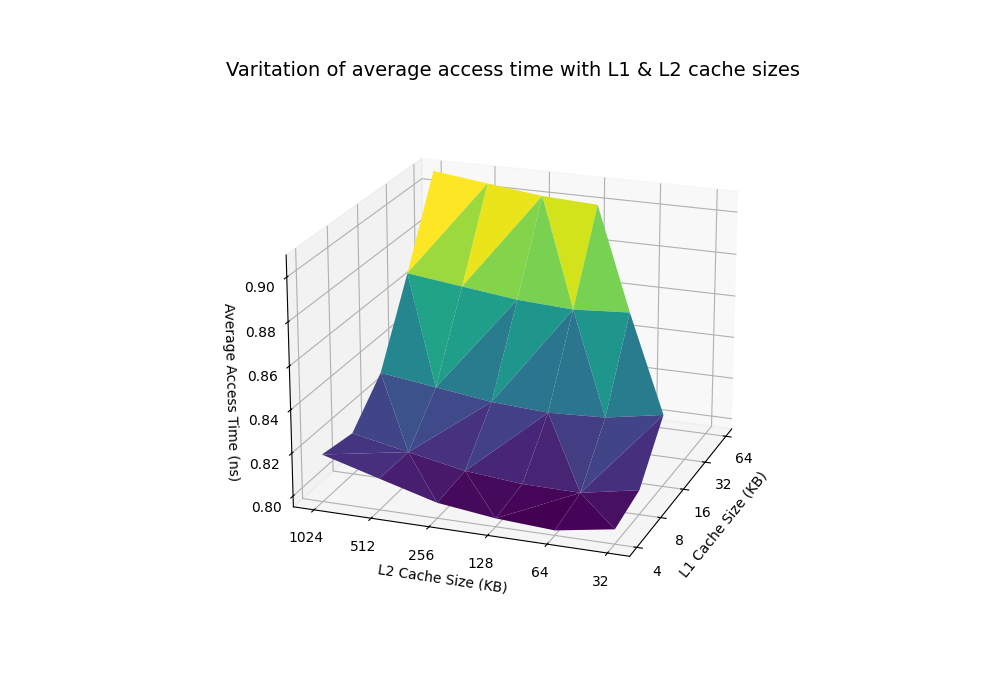
\includegraphics[width=0.9\textwidth]{figures/fig5/fig5.png}
        \centering
        \label{fig:fig5}
    \end{figure}

    Best average access time of 0.7972 ns is observed for a \textbf{4KB L1 cache along with a 64KB L2 Cache}. A 4KB L1 cache along with a 32KB L2 Cache, has an average access time of 0.8017, which is within 1\% of the best AAT. Further a reduction from 64KB to a 32KB L2 Caches decreases the total area by 26\%, from 0.3858 $\text{mm}^2$ to 0.2853 $\text{mm}^2$.
    
    \end{subsection}

   
    \begin{subsection}{Effect of L1 and L2 cache Size on Energy Delay Product}

        The surface plot below shows the Energy Delay Product for different L1 and L2 Cache Sizes. The L1 caches are taken as 4-way set associative and L2 caches as 8-way set associative. Blocksize is taken to be 32B in both caches.
    
        \begin{figure}[h!]
            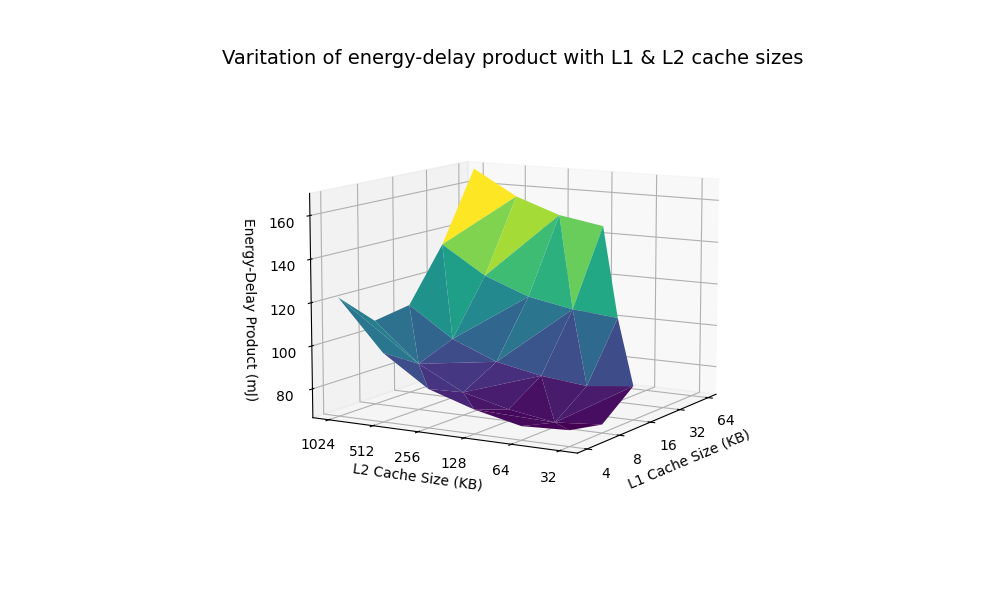
\includegraphics[width=0.9\textwidth]{figures/fig6/fig6.png}
            \centering
            \label{fig:fig6}
        \end{figure}
    
        Best energy delay product of 68.61 mJ is observed for a \textbf{8KB L1 cache along with a 64KB L2 Cache}.
        
    \end{subsection}
   
    \begin{subsection}{Effect of Victim Cache}

        The plot below shows the average access time for various configurations of L1 and victim cache along with a 8-way associative 256KB L2 cache. Block size is taken to be 32B in both caches.

        \begin{figure}[h!]
            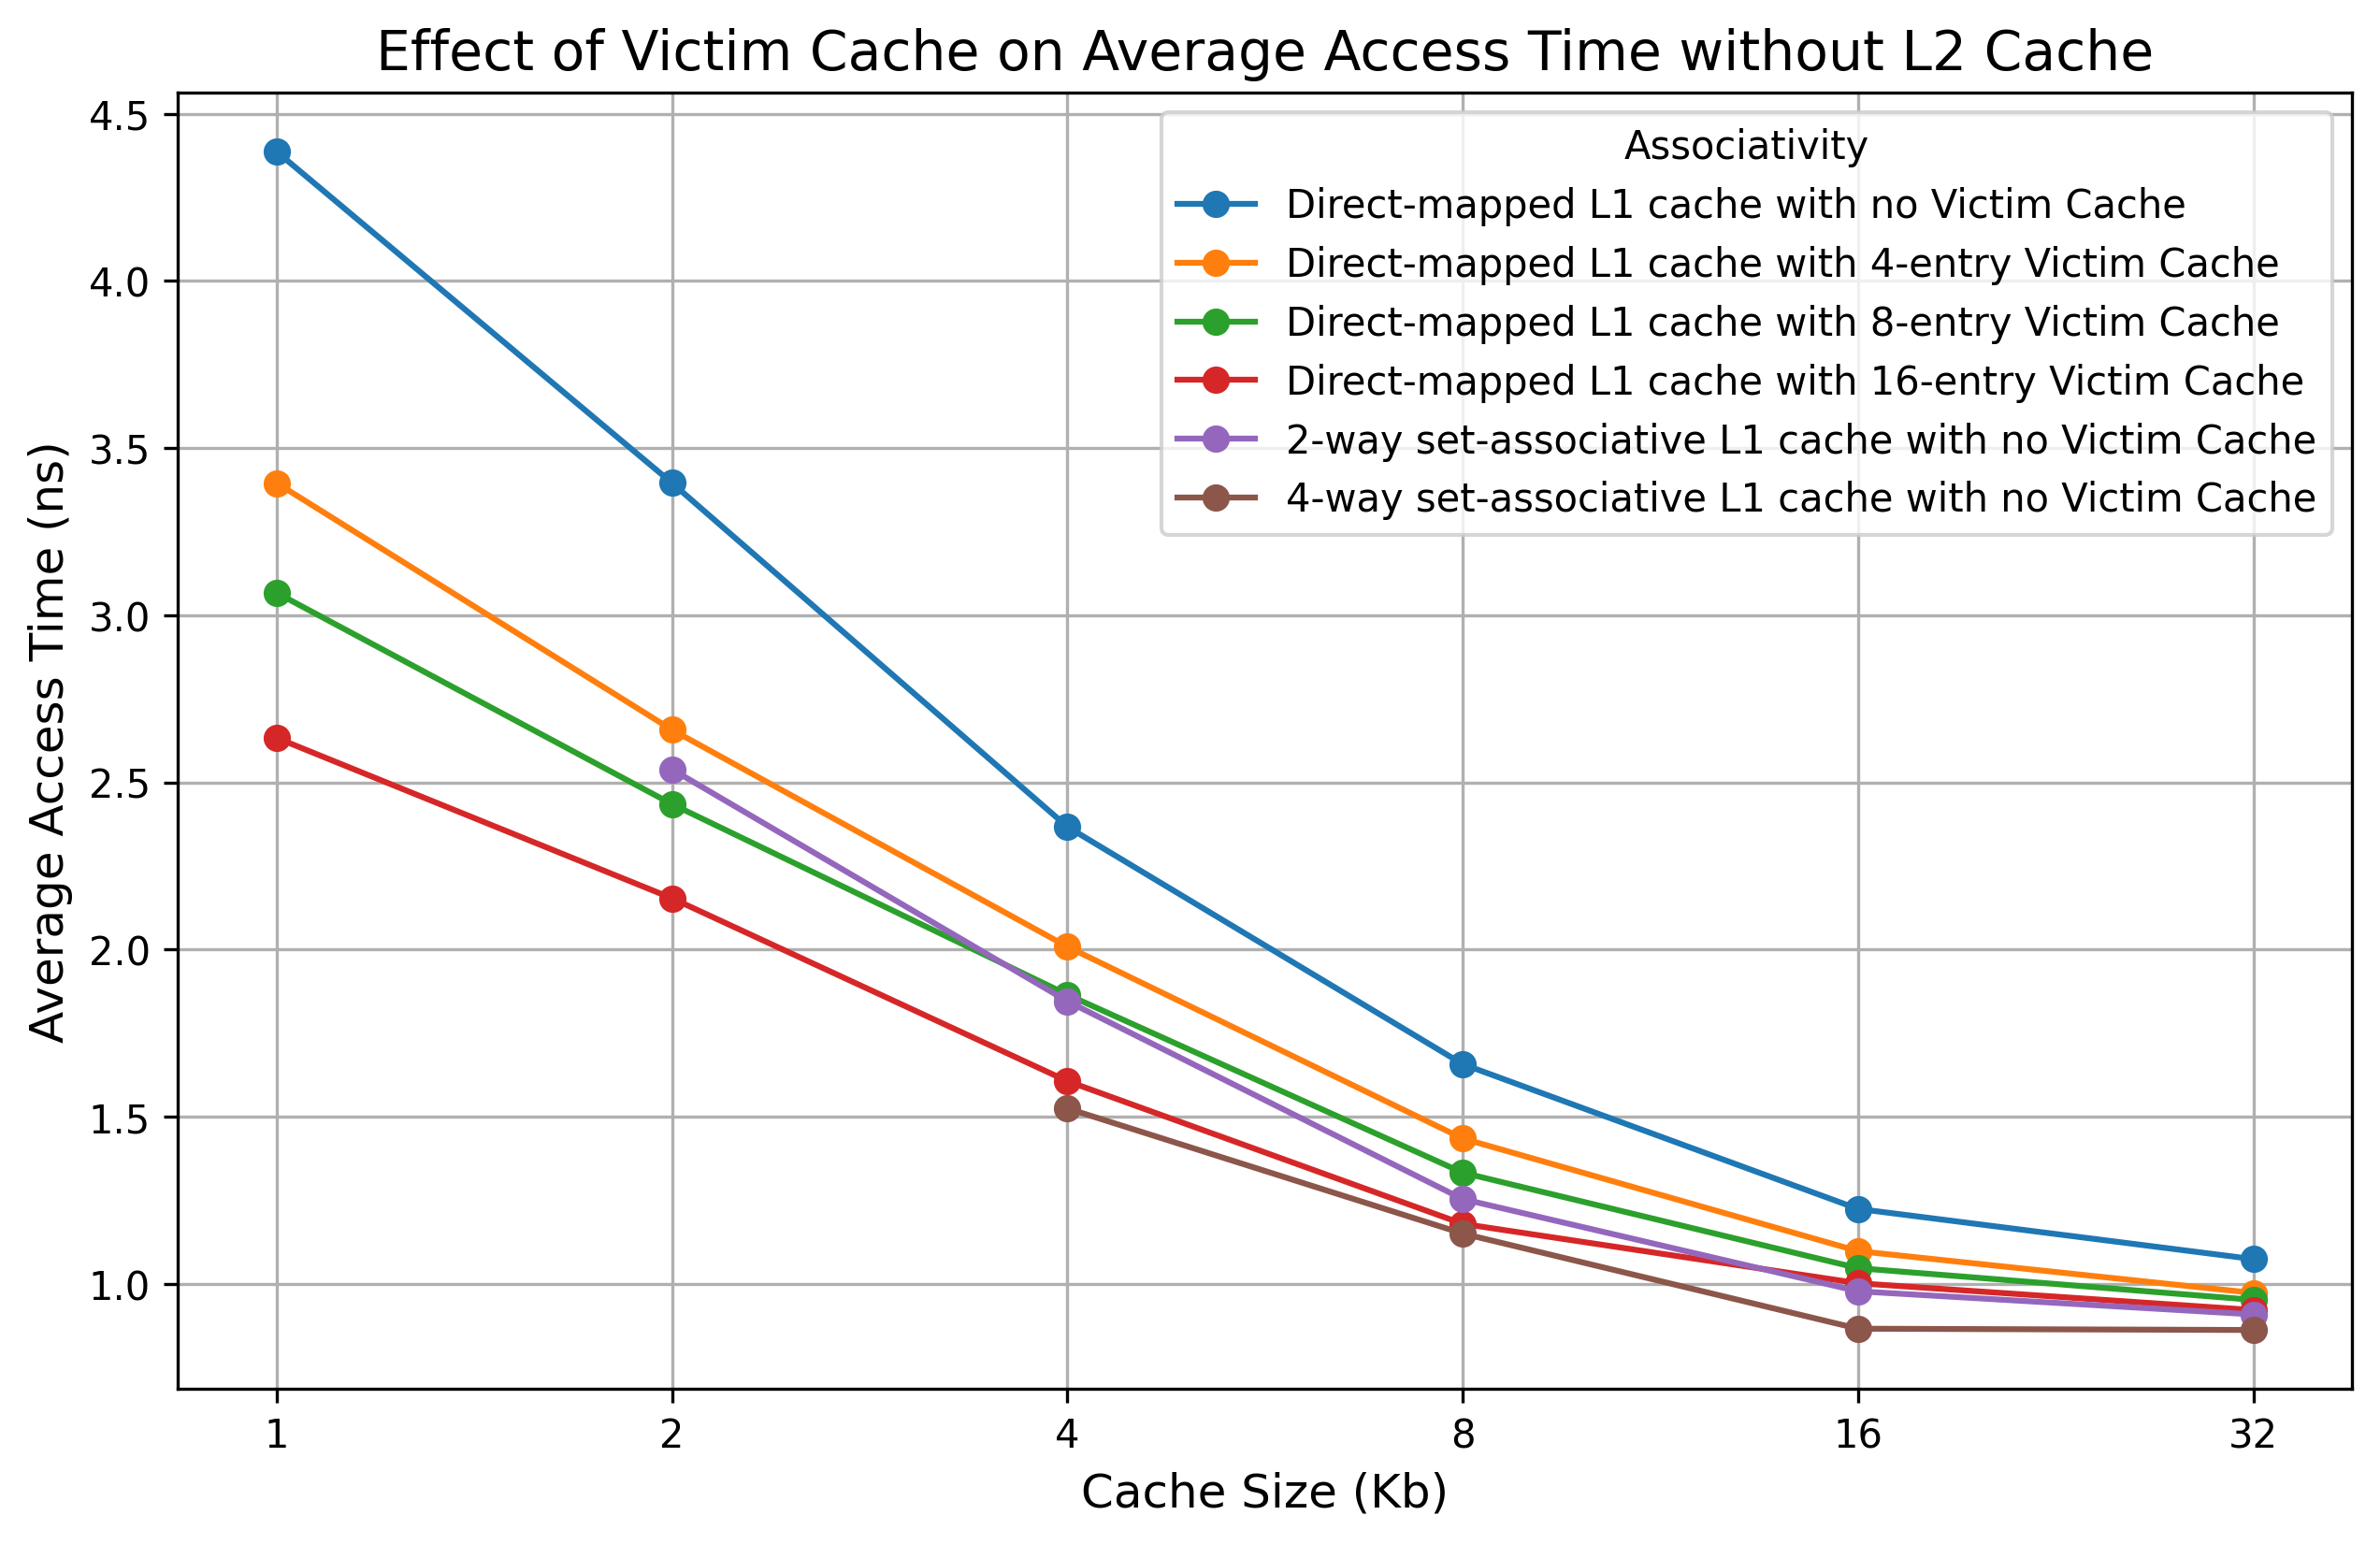
\includegraphics[width=0.9\textwidth]{figures/fig7/fig7.png}
            \centering
            \label{fig:fig7}
        \end{figure}

        \begin{itemize}
        \item As can be seen from the figure. All direct mapped L1 caches, with different victim cache sizes, perform better than 2-way and 4-way set associative L1 caches. This is because of the reduced miss penalty of the underlying L2 cache.
        \item A \textbf{2KB direct-mapped L1 cache with 16-entry victim cache} with this L2 configuration performs the best with an average access time of 0.7751 ns.
        \item A simple 1KB direct-mapped L1 cache has an average access time of 0.7861 ns, which is within 5\% of the average access time of the best configuration. Further this cache configuration (along with L2 cache) has an area of $1.1760 \text{mm}^2$ compared to  $1.1710 \text{mm}^2$ of the best configuration. 
        \end{itemize}
        
    \end{subsection}

\end{section}